% -----------------------------------------------------------------------------
% Resultados
% -----------------------------------------------------------------------------

\chapter{Result Analysis and Discussion - BNE}
\label{chap:Resultados-BNE}

%Cada capítulo deve conter uma pequena introdução (tipicamente, um ou dois parágrafos), em seção não numerada, que deve deixar claro o objetivo e o que será discutido no capítulo, bem como a organização do capítulo.

%\section{Título da seção}
%\label{sec:titSecResult}

%Inserir seu texto aqui...

%    Nesta parte da tese, utilizaremos 2500 grãos. O diâmetro médio do grão é $d = 1\pm 2.5\%$, distribuídos uniformemente. O diâmetro do intruso é de $D = 5$ vezes o diâmetro médio dos grãos. A densidade de todos os grãos é a mesma, e vale $\rho = 1/\pi$, e portanto a massa média dos grãos é de $m = 0,25$, exceto quando estiver ressaltado nas figuras. A constante de mola na direção normal é de $k_{n} = 1000$ e a tangencial é de $k_{t} = 750$. A atuação do amortecedor é no regime crítico ($\gamma = 2\sqrt{m k}$), e vale aproximadamente $\gamma = \sqrt{10}$. O atrito dos grãos valem $\mu = 0,5$, tanto entre grãos, quanto entre paredes, quando houver. O passo de tempo ($dt=pT$) vale aproximadamente $dt = \frac{1}{2000\sqrt{10}}$, utilizando a fração de $p=0,01$ do período de oscilação do modelo de contato massa mola $T = \sqrt{\frac{m}{k}}$. A largura da caixa é de $L = 37.5$ diâmetros de grão.

    In this Chapter we will present the results obtained from BNE simulations. These results were published in Reference \cite{Large-deviation_quantification_of_boundary_conditions_on_the_Brazil_nut_effect}, also present in Appendix \ref{appendix:BNE}. The parameters we used to simulate the system is 2500 grains, with average diameter $d$ = 1 $\pm$ 2.5\%, with uniform distribution, the intruder diameter $D$ = 5$d$. Grains and intruder density $\rho$ = 4/$\pi$, leading the average mass $m$ = 1, the spring constant in the normal direction $k_{n}$ = 1000 and the spring constant in the tangential direction $k_{t}$ = 750, the critical damping coefficient $\gamma$ = 2$\sqrt{m_r k_{n}}$, $m_r$ = $\frac{m_i m_j}{m_i + m_j}$, the friction coefficient $\mu$ = 0.5 between grain-grain contact, grain-intruder contact, grain-wall intruder contact and intruder-wall contact. The time step dt = $\frac{1}{100}\sqrt{\frac{m_r}{k_n}}$, the width $w$ = 37.5$d$, the gravity acceleration $g$ = 1. Any different parameter used is described properly in each corresponding Figure and in the text. As an example, Figure \ref{fig:BNE}.

%    Inicialmente, estudamos o sistema com paredes no fundo e nas laterais, formando uma caixa. Observamos, nestas simulações, correntes de convecção próximas às paredes.

\begin{figure}
    \centering
    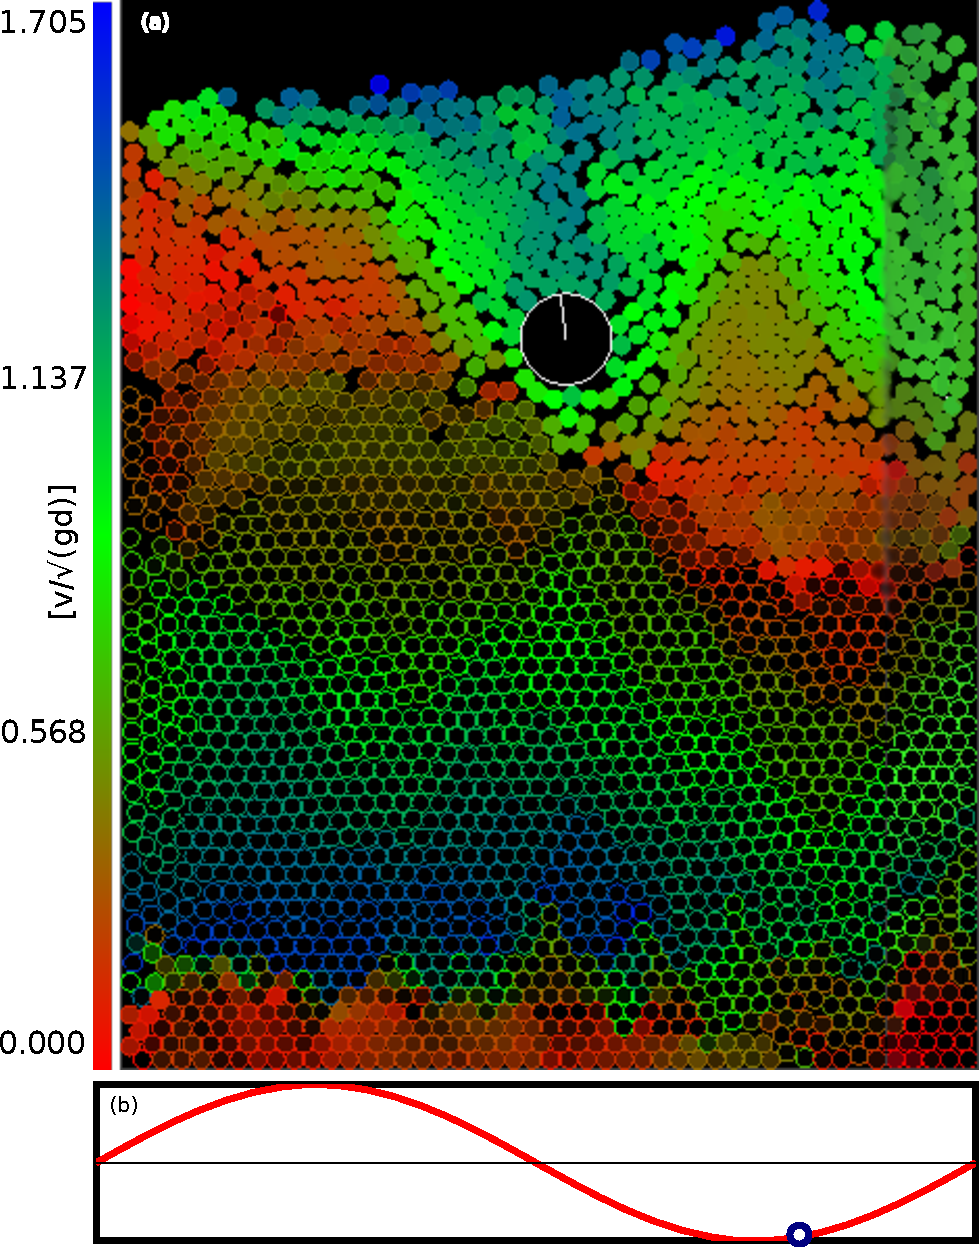
\includegraphics[width=0.65\textwidth]{04-figuras/BNE.pdf}
    \caption[BNE snapshot.]{In panel (a), a snapshot of the system lateral walls. Grains are represented by discs: hollow discs ($\textcolor{black}{\circ}$) are moving downward (with gravity) while filled ones ($\textcolor{black}{\bullet}$) are moving upward (against gravity). Color level shown at left side indicates the magnitude of the speed: red indicates no movement while blue indicates the maximum value for the speed. It is worth noting the inertia of the intruder accelerating the grains above him (bluish grains). It is also possible to observe the transition between the grains rising and falling in the reddish region around the intruder, a characteristic responsible for the granular ratchet effect. While the intruder easily displaces the grains on the way up, he is unable to move the grains that descend due to the steric exclusion. In panel (b) a sinusoidal displacement imposed to the substrate. This snapshot was taken after the minimum of the oscillation of the substrate, marked as a blue dot in this plot. Figure also present in \cite{Large-deviation_quantification_of_boundary_conditions_on_the_Brazil_nut_effect}.}
    \label{fig:BNE}
\end{figure}

    Initially, we studied the system with bottom and sidewalls, forming a box. In these simulations, we observed convection currents close to the walls. This convection currents are the main contribution to the rise of the intruder. The sequential position of the intruder in a single example is shown in Figure \ref{fig:BNE_intruderwalls}.

\begin{figure}
    \centering
    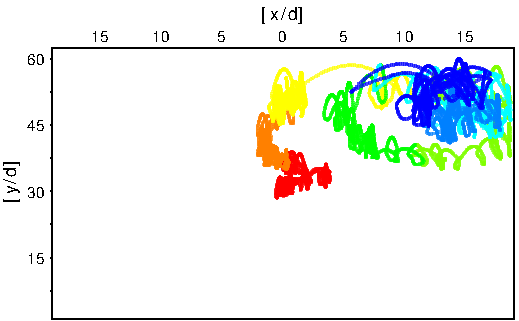
\includegraphics[width=0.65\textwidth]{04-figuras/BNE_PositionWalls.pdf}
    \caption[BNE with walls: sample of intruder positions.]{Sequential positions of the intruder $(x, y)$ taken at constant time intervals (0.316 $\sqrt{d/g}$), for a system with lateral frictional walls (fw). The shaken frequency $\omega$ = 0.256$\sqrt{d/g}$. $y$ = 0 indicates the box floor and the unities are in unities of the mean grain diameter. The change in colors indicates the time elapsed in the simulation, the red corresponds to the beginning of the simulation and the blue to the end.}
    \label{fig:BNE_intruderwalls}
\end{figure}

    The following Figures \ref{} show ascent profiles of the intruder.

\begin{figure}
    \centering
    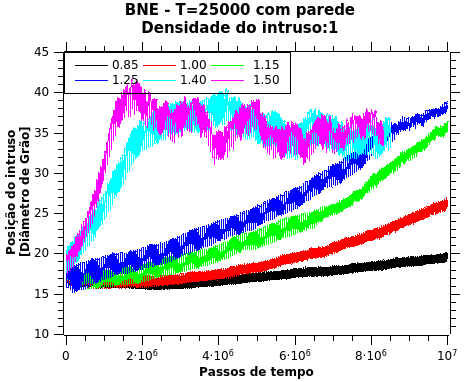
\includegraphics[width=0.65\textwidth]{04-figuras/BNE25000D1.png}
    \caption[BNE with frictional walls: $\rho_I/\rho_g$ = 1.]{Time series for intruder horizontal position at different $\Gamma$ for system with frictional walls (fw). The density $\rho_I/\rho_g$ = 1, with $\rho_I$ the density of the intruder and $\rho_g$ the density of the media. Simulations run until $...\sqrt{d/g}$. Figure also present in \cite{Large-deviation_quantification_of_boundary_conditions_on_the_Brazil_nut_effect}.}
    \label{fig:BNE25000_Parede}
\end{figure}

\begin{figure}
    \centering
    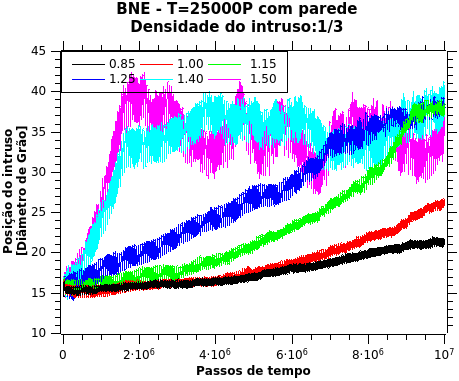
\includegraphics[width=0.65\textwidth]{04-figuras/BNE25000D1-3.png}
    \caption[BNE with frictional walls: $\rho_I/\rho_g$ = 1/3.]{Time series for intruder horizontal position at different $\Gamma$ for system with frictional walls (fw). The density $\rho_I/\rho_g$ = 1/3, with $\rho_I$ the density of the intruder and $\rho_g$ the density of the media. Simulations run until $...\sqrt{d/g}$.}
    \label{fig:BNE25000_Parede_Densidade1-3}
\end{figure}

\begin{figure}
    \centering
    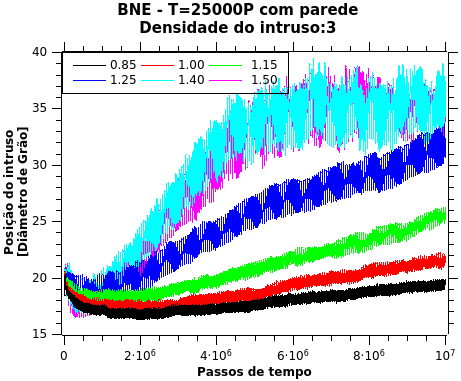
\includegraphics[width=0.65\textwidth]{04-figuras/BNE25000D3.png}
    [BNE with frictional walls: $\rho_I/\rho_g$ = 1.]{Time series for intruder horizontal position at different $\Gamma$ for system with frictional walls (fw). The density $\rho_I/\rho_g$ = 3, with $\rho_I$ the density of the intruder and $\rho_g$ the density of the media. Simulations run until $...\sqrt{d/g}$.}
    \label{fig:BNE25000_Parede_Densidade3}
\end{figure}

%    Percebemos que intrusos mais densos sobem mais lentamente que intrusos menos densos. Os tempos de subida, quando comparados, podem ser ordenados das figuras $\ref{fig:BNE25000_Parede_Densidade1-3} < \ref{fig:BNE25000_Parede} < \ref{fig:BNE25000_Parede_Densidade3}$. Assim como as correntes de convecção são mais intensas, o intruso sobe mais rapidamente e cai mais rapidamente, visto na amplitude de $\Gamma = 1,5$ para as figuras \ref{fig:BNE25000_Parede_Densidade1-3}, \ref{fig:BNE25000_Parede} e \ref{fig:BNE25000_Parede_Densidade3}, respectivamente.

    We saw that denser intruders rise more slowly than less dense intruders for all $\Gamma$. For this frequency, we saw the contrary predicted in the BNE, the denser would rise faster than the less dense. This effect may be a peculiar behavior for this frequency, or the density range we test. We also notice that the convection current is stronger the less dense the intruder is. As expected, the higher the $\Gamma$ the faster the ascent rate.

%    Quando retirado o atrito entre os grãos e as paredes, temos que o efeito da convecção no sistema diminui, ocasionando uma subida mais lenta que quando o atrito está presente. A figura \ref{fig:BNE25000_sem_Atrito_Parede} mostra a subida do intruso no sistema em que as paredes não possuem atrito.

    When frictionless walls (flw) are in play, we saw that convection decreases, causing a slower ascent rate, compared to fw. Figure \ref{fig:BNE2500_sem_Atrito_Parede} shows the intruder rise in a flw system, in opposition to the explanation in the Reference \cite{Inertia_in_the_Brazil_nut_problem}. For flw, we saw that $\Gamma$ = 0.85 was not able to rise, while fw rises with slow ascent rate.

\begin{figure}
    \centering
    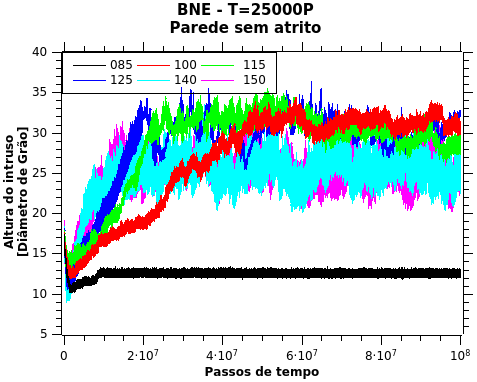
\includegraphics[width=0.65\textwidth]{04-figuras/BNE25000PsemAtrito.png}
    \caption[BNE with frictionless walls.]{Time series for intruder horizontal position at different $\Gamma$ for system with flw. The density $\rho_I/\rho_g$ = 1, with $\rho_I$ the density of the intruder and $\rho_g$ the density of the media.}
    \label{fig:BNE25000_sem_Atrito_Parede}
\end{figure}

%    Ao comparar os tempos de subida do sistema que possui atrito nas paredes (figura \ref{fig:BNE25000_Parede}) com o sistema que não possui atrito nas paredes (figura \ref{fig:BNE25000_sem_Atrito_Parede}), percebemos que o tempo de subida é maior, além de que o sistema que possui agitação menor que a gravidade não sobe, mostrando que um dos fatores que importam para o \textit{BNE} são as correntes de convecção formadas próximas das paredes.

    When comparing the rise times of fw (figure \ref{fig:BNE25000_Wall}) with flw (figure \ref{fig:BNE25000_without_Atrito_Wall}), we notice that the rise time is larger, and the system that has less agitation than gravity does not rise, showing that one of the factors that matter for the BNE are the convection currents formed close to the walls and the convection currents are enhanced by fw.

    We define the ascent rate as the difference between the initial position of the intruder to its highest position, then divide this difference by the time it takes to rise. Than we plot the ascent rate versus shaken frequency for each $\Gamma$.

\begin{figure}
    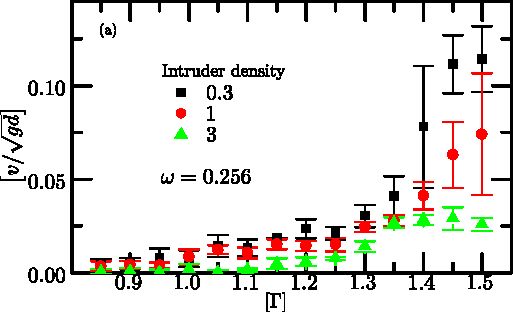
\includegraphics[width=0.65\linewidth]{04-figuras/BNE_FW_Density.pdf}
    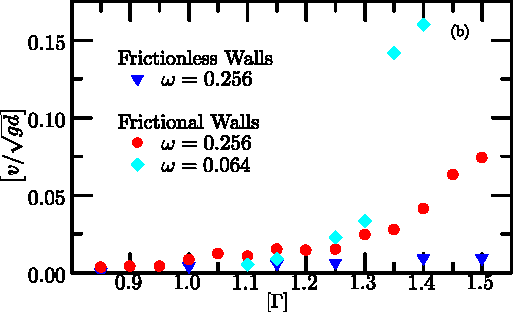
\includegraphics[width=0.65\linewidth]{04-figuras/BNE_W.pdf}
    \caption{In (a), the simulation was set to fw, width of 37.5d, shaken frequency of $0.256\sqrt{g/d}$, 2500 grains, and we have varied the intruder density, compared to the medium. In (b), a comparison between fw and flw and a change in frequency. Figure also present in \cite{Large-deviation_quantification_of_boundary_conditions_on_the_Brazil_nut_effect}.}
    \label{fig:BNE_walls}
\end{figure}

%    Quando retiramos o atrito do sistema, o intruso chega ao fundo do sistema, independente da amplitude de vibração. A figura \ref{fig:BNE25000_sem_Atrito} exibe o comportamento do intruso para o sistema sem atrito.

    When no friction is present on the system, the intruder sinks to the bottom, independently from the amplitude of the vibration. Figure \ref{fig:BNE25000_sem_Atrito} exhibits the height of the intruder in frictionless system. As expected, no friction on the system causes no BNE, and the simulations we have performed shows that the intruder sinks to bottom. We are not going to count this fact as a RBNE, since only friction has changed.

\begin{figure}
    \centering
    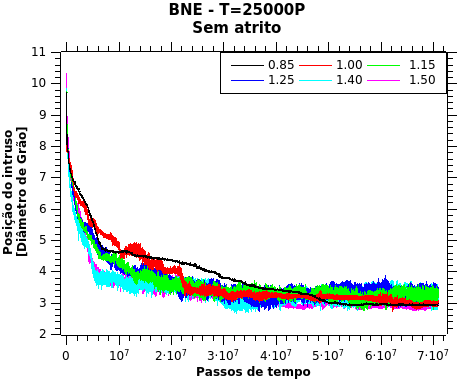
\includegraphics[width=0.65\textwidth]{04-figuras/BNE25000semAtrito.png}
    \caption[Frictionless grains and walls.]{Time series for the intruder's fall in no friction system. Independent of $\Gamma$, the intruder sinks to the bottom.}
    \label{fig:BNE25000_sem_Atrito}
\end{figure}

    If instead of having sidewalls, we replace them with a periodic boundary condition (pbc), we could have the intruder crossing from one side to another, something impossible to do with walls, but also we expect to do not have the sidewalls effect, like convection currents. As an example of the intruder position through time, Figure \ref{fig:BNE_intruderpbc}. A difference between fw and pbc is the fact that the intruder can follow the convection current in fw and sink a little bit, while in pbc it does not sink in the media.

\begin{figure}
    \centering
    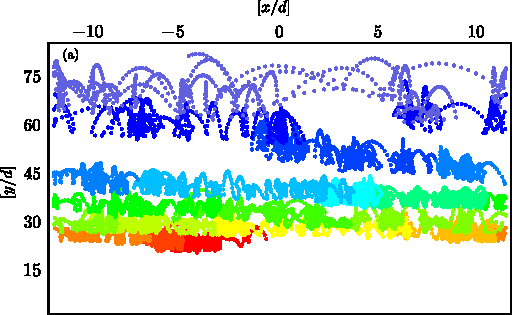
\includegraphics[width=0.65\textwidth]{04-figuras/BNE_PositionPBC.pdf}
    \caption[BNE with periodic boundary: sample of intruder positions.]{Sequential positions of the intruder $(x, y)$ taken at constant time intervals (0.316 $\sqrt{d/g}$), for a system with pbc. The shaken frequency $\omega$ = 0.213$\sqrt{d/g}$. $y$ = 0 indicates the box floor and the unities are in unities of the mean grain diameter. The change in colors indicates the time elapsed in the simulation, the red corresponds to the beginning of the simulation and the blue to the end. The width of the pbc in this sequential positions is $w$ = 25$d$. Figure also present in \cite{Large-deviation_quantification_of_boundary_conditions_on_the_Brazil_nut_effect}.}
    \label{fig:BNE_intruderwalls}
\end{figure}

%    Se ao invés de retirarmos o atrito, retirarmos as paredes laterais formando uma condição periódica de contorno de largura $28$ diâmetros de grão, verificaremos que o \textit{BNE} não acontece para o período de vibração de $25000$ passos de tempo, como mostrado na figura \ref{fig:BNE25000_Contorno}.

    The as an example of pbc intruder ascent temporal profile, Figure \ref{fig:BNE30000_Contorno}. Two differences are present here, if we compare fw and pbc: the ascent time of the intruder for each $\Gamma$ and the shaken frequency. At the same frequency applied to the fw, the pbc did not rise at all. The response is shown in Figure \ref{fig:BNE_resonance}.

%    Já no caso de períodos maiores, o BNE ocorre. A figura \ref{fig:BNE30000_Contorno} exemplifica o \textit{BNE} ocorrendo com condição periódica de contorno e período de vibração de $30000$ passos de tempo.

\begin{figure}
    \centering
    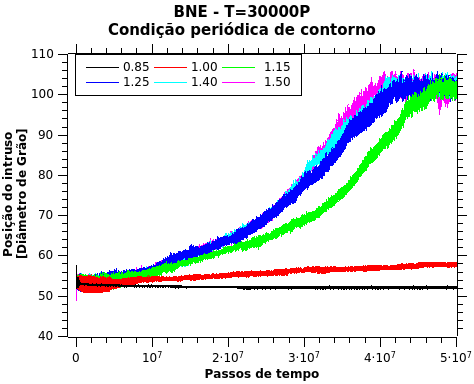
\includegraphics[width=0.65\textwidth]{04-figuras/BNE30000Contorno.png}
    \caption[BNE with periodic boundary: time series.]{Time series for intruder horizontal position at different $\Gamma$ for system with pbc. The density $\rho_I/\rho_g$ = 1, with $\rho_I$ the density of the intruder and $\rho_g$ the density of the media. The value of $\omega$ = 0.213. Figure also present in \cite{Large-deviation_quantification_of_boundary_conditions_on_the_Brazil_nut_effect}.}
    \label{fig:BNE30000_Contorno}
\end{figure}

%    Na figura \ref{fig:BNE30000_Contorno}, percebemos que acelerações menores que a gravidade não fazem o intruso ascender, enquanto acelerações próximas da gravidade tem um movimento de ascensão lento e em saltos. Por não haver paredes, as correntes de convecção não se formam no sistema, o que faz com que o intruso atinja o topo e não desça mais.

    In Figure \ref{fig:BNE30000_Contorno}, we see that accelerations less than gravity do not cause the intruder to ascend, while accelerations close to gravity have a slow, jumping ascent. Because there are no sidewalls, convection currents do not form in the system, which causes the intruder to reach the top and not descend any further. 

\begin{figure}
    \centering
    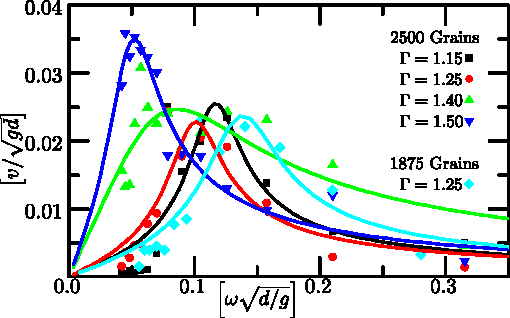
\includegraphics[width=0.65\textwidth]{04-figuras/BNE_ResonancePBC.pdf}
    \caption[BNE with periodic boundary: resonance.]{Intruder ascent rate $v$ curves for various normalized external accelerations $ \Gamma $, for the pbc case. $\Gamma = 1.15$ and $2500$ grains is in $\textcolor{black}{\blacksquare}$, $\Gamma = 1.25$ and $2500$ grains is in $\textcolor{red}{\bullet}$, $\Gamma = 1.40$ and $2500$ grains is in $\textcolor{green}{\blacktriangle}$, $\Gamma = 1.50$ and $2500$ grains is in $\textcolor{blue}{\blacktriangledown}$, $\Gamma = 1.25$ and $1875$ grains is in $\textcolor{cyan}{\Diamondblack}$, all with $37.5d$ wide. Figure also present in \cite{Large-deviation_quantification_of_boundary_conditions_on_the_Brazil_nut_effect}.}
    \label{fig:BNE_resonance}
\end{figure}

    Figure \ref{fig:BNE_resonance} shows us that the ascent rate changes with the applied frequency, and as sudden the intruder ascent to the top, we propose that the behavior of the BNE in pbc could be modelled as a resonant system, since that dependency on $\omega$ is expected for a typical resonant system. Then, in analogy, the system behaves like a forced damped harmonic oscillator, with the response in the element that dissipates energy. The equation of a linear damped harmonic oscillator is:
%
\begin{equation}
    \frac{d^2 y}{d t^2} + 2 \zeta \omega_0 \frac{d y} {d t} + \omega_0^2 y = \Gamma \sin(\omega t) ~,  
\end{equation}
%
where $\omega_0$ is the natural frequency of the system, $\zeta$ is the damping ratio, a parameter of the fitting function. The solution to this equation can be written is several forms depending on the element over which is measured the response. Considering the resonant system in analogy to a mass-spring-damper system, if we measure the transfer function over the damper element, which represents the ascent rate of the intruder, the solution for the gain reads:
%
\begin{equation}
    G(\omega) = \frac{2 \zeta \omega_0 \omega }{ \sqrt{(2 \zeta \omega_0 \omega)^2 + (\omega_0^2 - \omega^2)^2 }}~,
    \label{equ:TF}
\end{equation}
%
that we have used to fit the data in Figure \ref{fig:BNE_resonance}. Note the bell shape of the fitting curves, analogous to the sharpness curve for the amplitude magnitude typical in traditional resonance analysis. We use the fact that pbc systems does not have convection current, and the main effect to ascent the intruder is the ratchet effect.

    The data could be collapsed around the fitted parameter $\omega_0$ and results in the curve shown in Figure \ref{fig:BNE_collapse}. The fitting parameters are shown in Figure \ref{fig:BNE_fit_parameters}. Even harder grains obeys this trend. The dynamics of the resonance does not follow exactly the linear approximation, as we can observe in log-log scale, but near the peak the adjust is good.

\begin{figure}
    \centering
    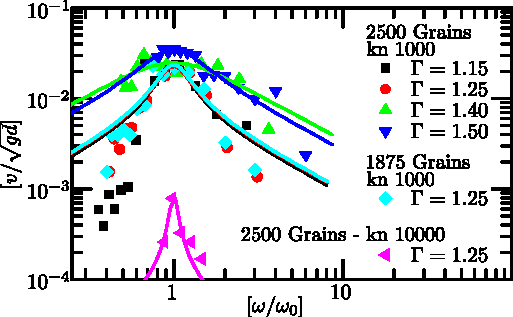
\includegraphics[width=0.65\textwidth]{04-figuras/BNE_Collapse.pdf}
    \caption[BNE with periodic boundary: resonance collapse.]{Collapse of the measured values. The data points are collapsed for all simulations with pbc. The fit can cover the ascent rate for different parameters, like stiffness $k_n$, normalized acceleration $\Gamma$, and the column above the intruder $h$. Figure also present in \cite{Large-deviation_quantification_of_boundary_conditions_on_the_Brazil_nut_effect}.}
    \label{fig:BNE_collapse}
\end{figure}

\begin{figure}
    \centering
    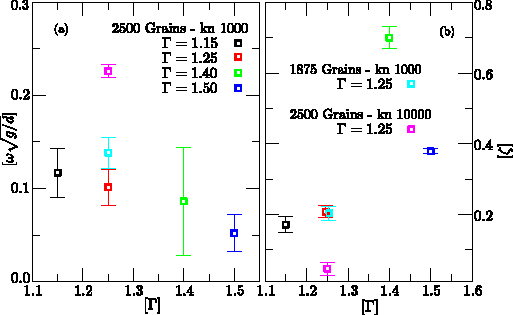
\includegraphics[width=0.65\textwidth]{04-figuras/BNE_Fit.pdf}
    \caption[BNE with periodic boundary: resonance fitting parameters.]{Fit of the parameters of using Equation (\ref{equ:TF}). In (a), the fitted natural frequency $\omega_0$ shows little dependence with $\Gamma$. In (b), the dissipation parameter shows agreement within the error bars to a constant value. Figure also present in \cite{Large-deviation_quantification_of_boundary_conditions_on_the_Brazil_nut_effect}.}
    \label{fig:BNE_collapse}
\end{figure}

    The damping effect $\zeta$ in the fit does not relate to the damping factor $\gamma$ (or restitution coefficient $\epsilon$) of the grains contact, once the $\gamma$ is critical and would lead to dissipation of energy enough to resonance does not happen in the contact interaction. A further investigation into this system linking force balance or energy balance to the proposed resonance is needed. We propose a scale in the frequency $\omega \propto \sqrt{k_n^3}/h$ while the ascent rate $v \propto \frac{d}{h g}\left(\sqrt{\frac{k_n/m}{\Gamma}}\right)^3$, where $k_n$ is the stiffness of the grains, $h$ is the difference between the top layer of grains and the intruder position, $d$ is the grain diameter, $g$ is the gravity, $m$ is the mass of the grains, and $\Gamma$ is the dimensionless shaken acceleration compared to the gravity.

\begin{figure}
    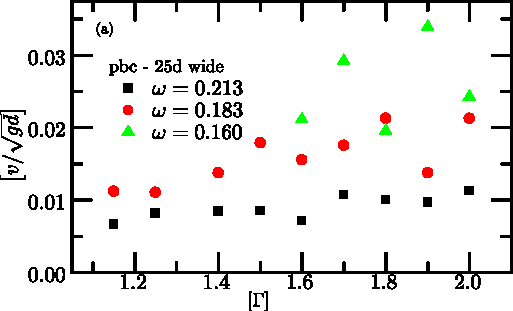
\includegraphics[width=0.65\linewidth]{04-figuras/BNE_PBC25.pdf}
    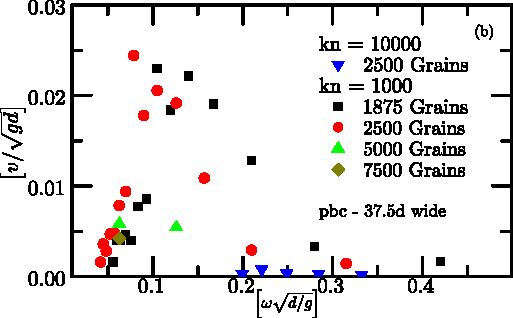
\includegraphics[width=0.65\linewidth]{04-figuras/BNE_PBC37.pdf}
    \caption[BNE with periodic boundary: 25$d$ and 37.5$d$.]{In (a), 25d wide in pbc. Increase $\Gamma$ leads to increase ascent rate. In (b) 37.5 wide in pbc. Figure also present in \cite{Large-deviation_quantification_of_boundary_conditions_on_the_Brazil_nut_effect}.}
    \label{fig:BNE_pbc}
\end{figure}

    And at least comparison in Figure \ref{fig:BNE_pbc}, another exploration on the parameters: width of 25$d$ and different number of grains in width of 37.5$d$, all in pbc.

    To reinforce the idea of the resonance, we analyse the fluctuation properties of the ratchet effect using Large Deviation Function (LDF) \cite{Symmetry_properties_of_the_large-deviation_function_of_the_velocity_of_a_self-propelled_polar_particle, Large_Deviations_in_Physics}. We quantify the fluctuations of the ascent rate distribution of the intruder measuring the normalized  $W_{\tau}$ as:
%
\begin{equation}
    W_{\tau}(t) = \frac{1}{\tau} \int_t^{t+\tau} \frac{v(t')}{\left<v\right>} dt'~, 
\end{equation}
%
where $v(t)$ is the intruder vertical velocity at time $t$ and $\left< \cdot \right>$ denotes the average over $[0,t+\tau]$. Next, we have calculated $P(W_{\tau})$, the density probability function of $W_\tau$, and obtained the RF at the limit
%
\begin{equation}
    RF(W_\tau) = -\lim_{\tau \rightarrow \infty} \frac{1}{\tau} \ln P(W_\tau)~.
\end{equation}

    We could collapse the curves for long range integration times, when we can see the BNE regime acting in the system. The short time integration did not collapse, once the predominant dynamic is the external oscillation. Figure \ref{fig:LDFgamma} shows the LDF in fw and pbc. When fw are in play, the asymmetry between falling and rising is pronounced, shown with the metric $P(W_{\tau})$ in Figure \ref{fig:LDFgamma}(b). On the other hand, when pbc is consider, the asymmetry of upward and downward is only observed on a high value of $\tau$, Figure \ref{fig:LDFgamma}(d). The $RF$ reaches its value in small $W_{\tau}$ for fw, Figure \ref{fig:LDFgamma}(a), while only long values of $W_{\tau}$ exhibit larger jumps in pbc.

\begin{figure}
    \centering
    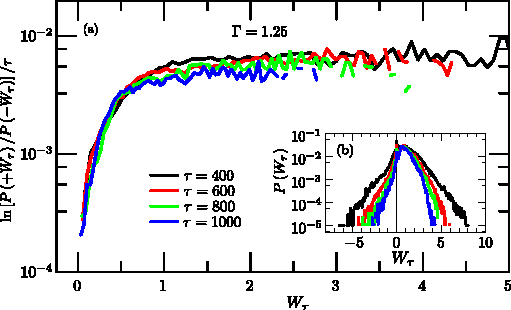
\includegraphics[width = 0.49\linewidth]{04-figuras/BNE_LDF_FW.pdf}
    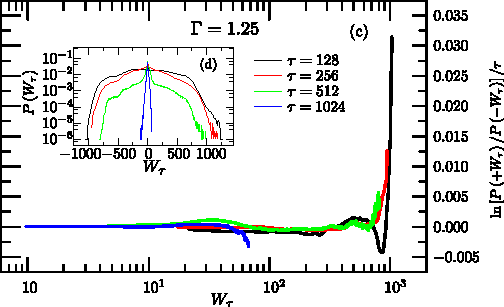
\includegraphics[width = 0.49\linewidth]{04-figuras/BNE_LDF_PBC.pdf}
    \caption[BNE with periodic boundary: large deviation.]{Inset: $P(W_\tau)$ for $\Gamma = 1.25$ and several values of $\tau$ as shown in the legends, for both systems: with frictional walls at left and pbc at right. Main panels: collapse of the RF function calculated for $\Gamma = 1.25$, and several values of $ \tau$.  Data collapse was performed by dividing the ratio between upward and downward probabilities by the integration time $\tau$. For the range of integration times considered, a remarkable collapse is observed. The frictional walls case is shown at left and pbc at right panel. Observe that distributions for pbc are much more symmetric than those for fw, which lean strongly to the positive side. Figure also present in \cite{Large-deviation_quantification_of_boundary_conditions_on_the_Brazil_nut_effect}.}
    \label{fig:LDFgamma}
\end{figure}

%    No próximo capítulo, descreveremos os modos de transporte de grãos quando arrastados por um fluido.

    Next Chapter we describe the techniques to simulate the fluid.
